\documentclass{beamer}

\usepackage[utf8x]{inputenc}
\usepackage[OT4]{fontenc}

\setbeamertemplate{navigation symbols}{}

\usetheme[lang=pl,pasek=pasek2]{pwr}

\usepackage{ragged2e}
\usepackage{hyphenat}
\usepackage{hyperref}
\usepackage{booktabs}
\usepackage{listings}
\usepackage{multibib}

\usepackage{tikz}

\usetikzlibrary{arrows}
\usetikzlibrary{automata}
\usetikzlibrary{backgrounds}
\usetikzlibrary{decorations}

\usepackage{amsmath}
\usepackage{amsfonts}
\usepackage{amsthm}

\usepackage{highlight/pythonhighlight}

\title{
    Design and implementation issues \linebreak
    of a computer algebra system \linebreak
    in an interpreted, dynamically typed \linebreak
    programming language
}

\author{Mateusz Paprocki \texttt{<mattpap@gmail.com>}}
\institute[PWR]{Wrocław University of Technology}
\date{\today}

\newenvironment{jblock}[1]{
    \begin{block}{#1}\justifying\nohyphens
}{
    \end{block}
}

\setbeamercovered{transparent}

\begin{document}

\begin{frame}[plain,t]
    \maketitle
\end{frame}

\begin{frame}
    \frametitle{Introduction}
    \framesubtitle{}

    \begin{center}
        \structure{Design} and \structure{implementation} issues \linebreak
        of a \structure{computer algebra system} \linebreak
        in an \structure{interpreted}, dynamically typed \linebreak
        programming language
    \end{center}

    \begin{itemize}
        \item supervisor: \structure{dr inż. Krzysztof Juszczyszyn}
        \item language: \structure{English}
    \end{itemize}
\end{frame}

\begin{frame}
    \frametitle{Plan of presentation}

    \begin{itemize}
        \item Remainder of the previous talk
        \item Multi--level structure
        \item Implemented algorithms
        \item Ground types
        \item Using Cython
        \item Future plans
    \end{itemize}
\end{frame}

\begin{frame}
    \frametitle{Thesis gloals}
    \framesubtitle{What I would like to achieve}

    Design and implement \structure{computer algebra module} for SymPy:
    \begin{itemize}
        \item conform SymPy's goals
        \pause
        \item introduce multi--level structure
        \pause
        \item multiple ground types
        \pause
        \item utilize \structure{pure mode} Cython
        \pause
        \item \ldots
    \end{itemize}
\end{frame}

\begin{frame}[fragile]
    \frametitle{Multi--level structure}
    \framesubtitle{}

    \begin{python}
>>> f3 = x**10 - 1
>>> %timeit factor_list(f3)
100 loops, best of 3: 5.57 ms per loop

>>> f2 = Poly(x**10 - 1, x, domain='ZZ')
>>> %timeit f2.factor_list()
100 loops, best of 3: 2.15 ms per loop

>>> f1 = DMP([mpz(1), mpz(0), mpz(0), mpz(0), mpz(0),
... mpz(0), mpz(0), mpz(0), mpz(0), mpz(0), mpz(-1)], ZZ)
>>> %timeit f1.factor_list()
100 loops, best of 3: 1.90 ms per loop

>>> f0 = [mpz(1), mpz(0), mpz(0), mpz(0), mpz(0),
... mpz(0), mpz(0), mpz(0), mpz(0), mpz(0), mpz(-1)]
>>> %timeit dup_factor_list(f0, ZZ)
100 loops, best of 3: 1.88 ms per loop
    \end{python}
\end{frame}

\begin{frame}
    \frametitle{Implemented algorithms}
    \framesubtitle{Only most remarkable cases here}

    \begin{itemize}
        \item square--free decomposition
            \begin{itemize}
                \item Yun
            \end{itemize}
        \item factorization into irreducibles
            \begin{itemize}
                \item finite fields
                    \begin{itemize}
                        \item Berlekamp, Shoup, Zassenhaus
                    \end{itemize}
                \item other domains
                    \begin{itemize}
                        \item Zassenhaus, Wang
                    \end{itemize}
            \end{itemize}
        \item functional decomposition
            \begin{itemize}
                \item Landau--Zippel
            \end{itemize}
        \item Gr\"{o}bner bases
            \begin{itemize}
                \item Buchberger
            \end{itemize}
        \item root isolation
            \begin{itemize}
                \item continued fractions, Collins--Krandick
            \end{itemize}
    \end{itemize}
\end{frame}

\begin{frame}[fragile]
    \frametitle{Ground types}
    \framesubtitle{An introduction}

    \begin{python}
In [1]: from sympy.polys.algebratools import ZZ_python

In [2]: ZZ
Out[2]: ZZ
In [3]: ZZ.dtype
Out[3]: <built-in function mpz>

In [4]: zz = ZZ_python()

In [5]: zz
Out[5]: ZZ
In [6]: zz.dtype
Out[6]: <type 'int'>

In [7]: zz.rep = 'ZZpy'

In [8]: Poly(x**10 - 1, domain=zz)
Out[8]: Poly(x**10 - 1, x, domain='ZZpy')
    \end{python}
\end{frame}

\begin{frame}
    \frametitle{Ground types}
    \framesubtitle{Benchmark: small coefficients}

    \begin{center}
        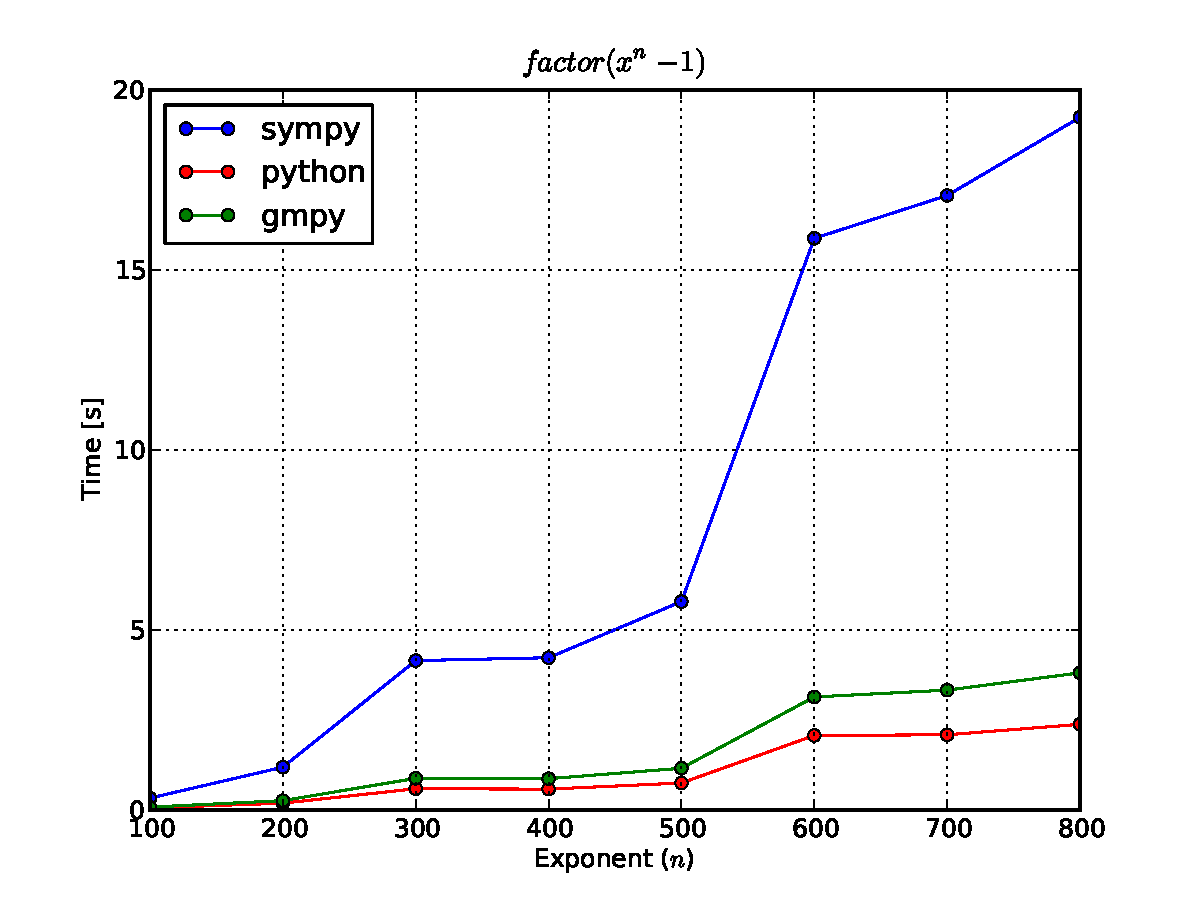
\includegraphics[scale=0.45]{images/ground-factor-small.pdf}
    \end{center}
\end{frame}

\begin{frame}
    \frametitle{Ground types}
    \framesubtitle{Benchmark: large coefficients}

    \begin{center}
        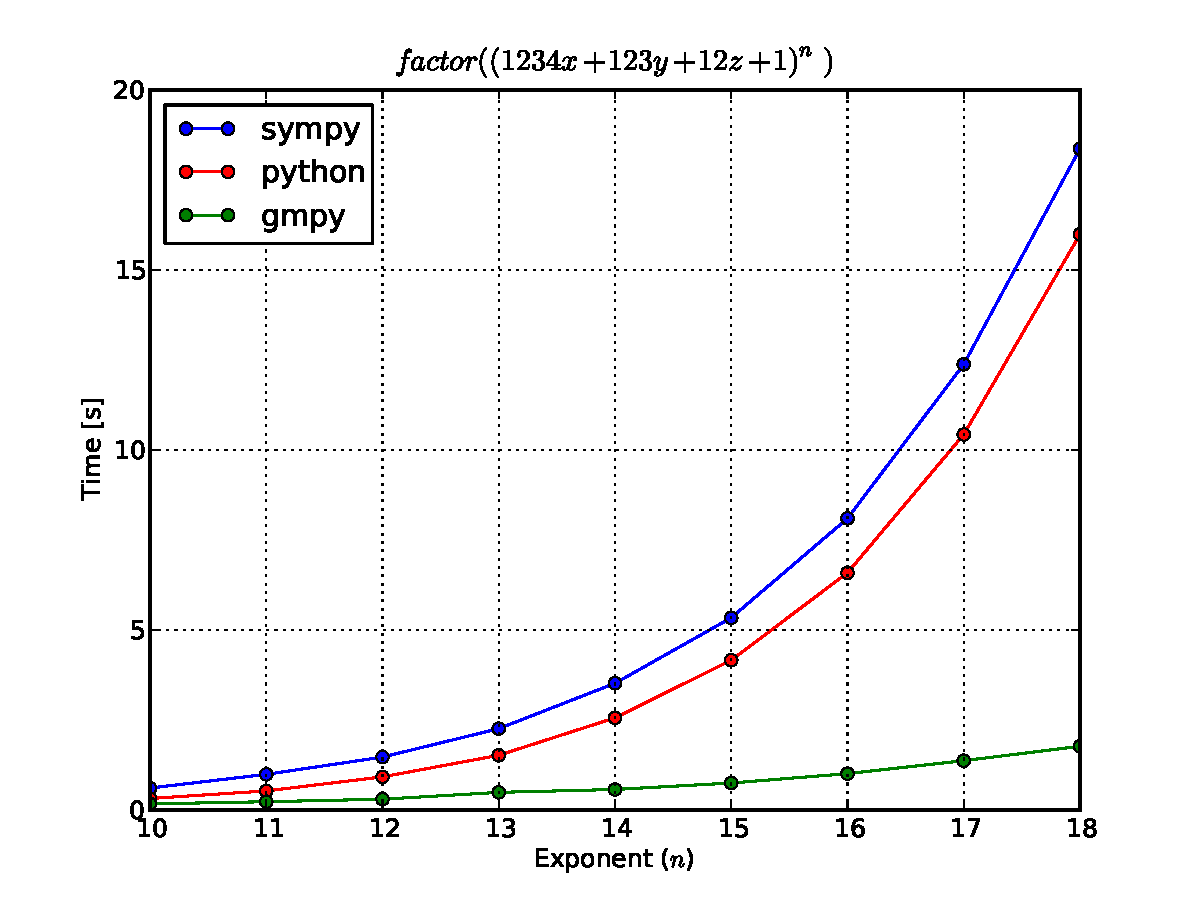
\includegraphics[scale=0.45]{images/ground-factor-large.pdf}
    \end{center}
\end{frame}

\begin{frame}
    \frametitle{Polynomial representations}
    \framesubtitle{An introduction}

    \begin{itemize}
        \item dense representation
            \begin{itemize}
                \item list of list
                \begin{equation*}
                    [[\ldots], [\ldots], \ldots, [\ldots]]
                \end{equation*}
            \end{itemize}
        \item sparse representation
            \begin{itemize}
                \item dictionary
                \begin{equation*}
                    [(M_n, c_n), (M_{n-1}, c_{n-1}) \ldots, (M_0, c_0)]
                \end{equation*}
            \end{itemize}
    \end{itemize}
\end{frame}

\begin{frame}
    \frametitle{Polynomial representations}
    \framesubtitle{Benchmark: 100\% dense exponentiation}

    \begin{center}
        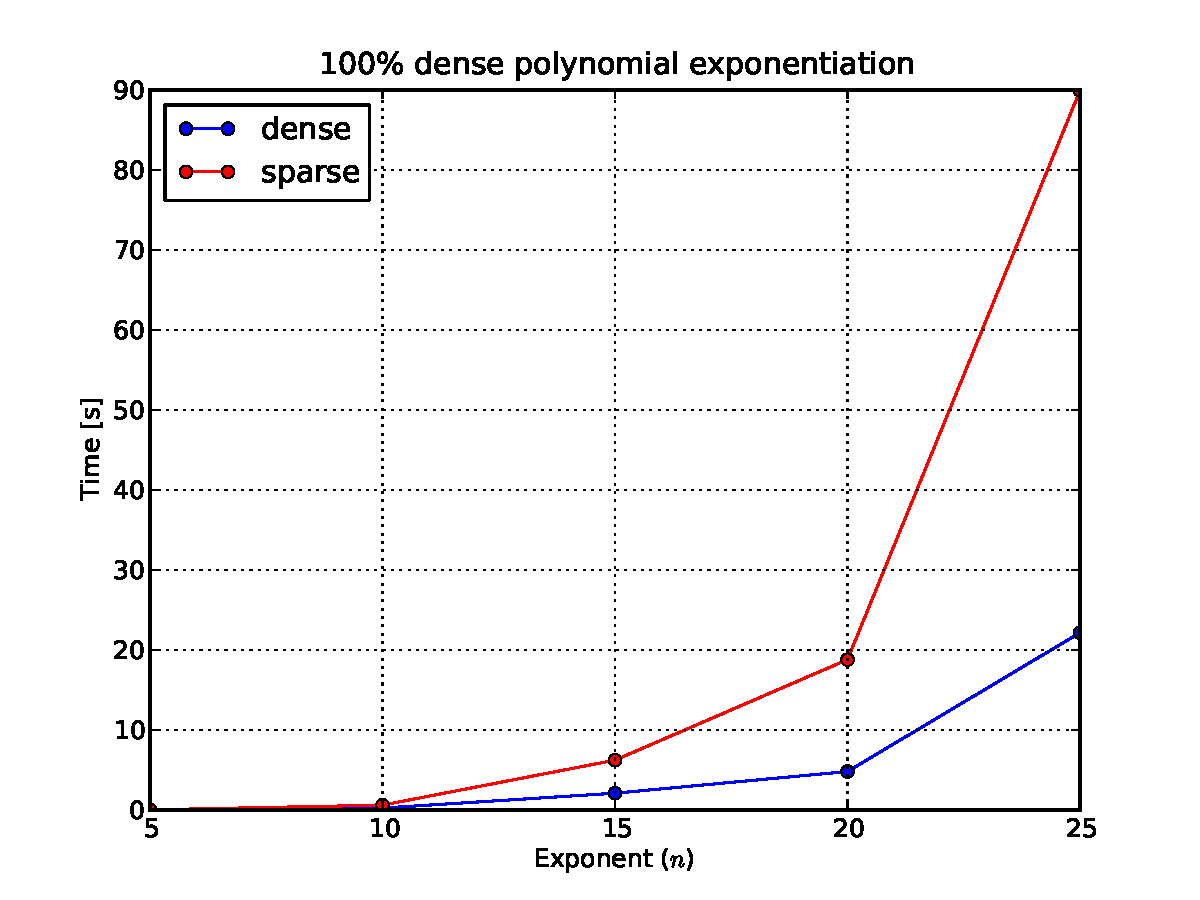
\includegraphics[scale=0.45]{images/100-dense-power.pdf}
    \end{center}
\end{frame}

\begin{frame}
    \frametitle{Polynomial representations}
    \framesubtitle{Benchmark: 50\% dense exponentiation}

    \begin{center}
        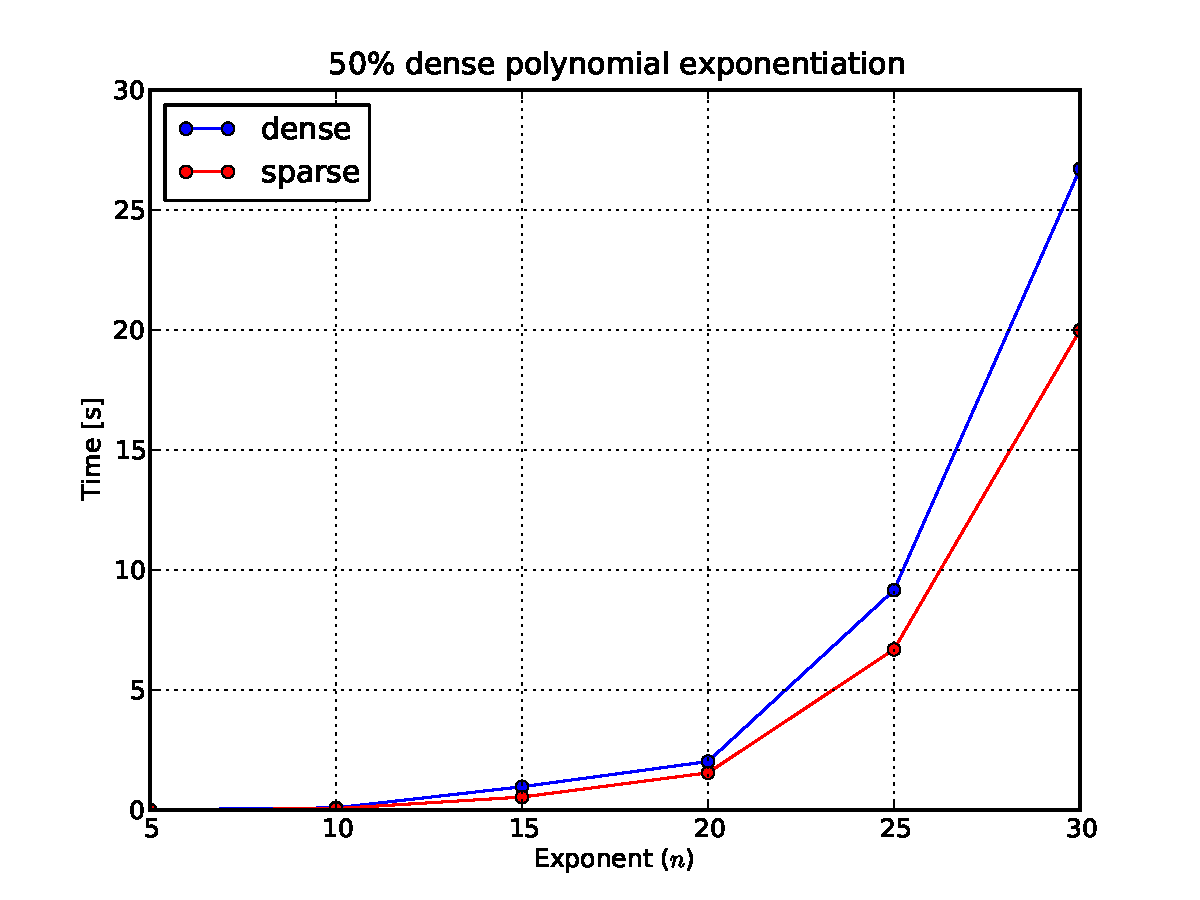
\includegraphics[scale=0.45]{images/50-dense-power.pdf}
    \end{center}
\end{frame}

\begin{frame}
    \frametitle{Polynomial representations}
    \framesubtitle{Benchmark: sparse exponentiation}

    \begin{center}
        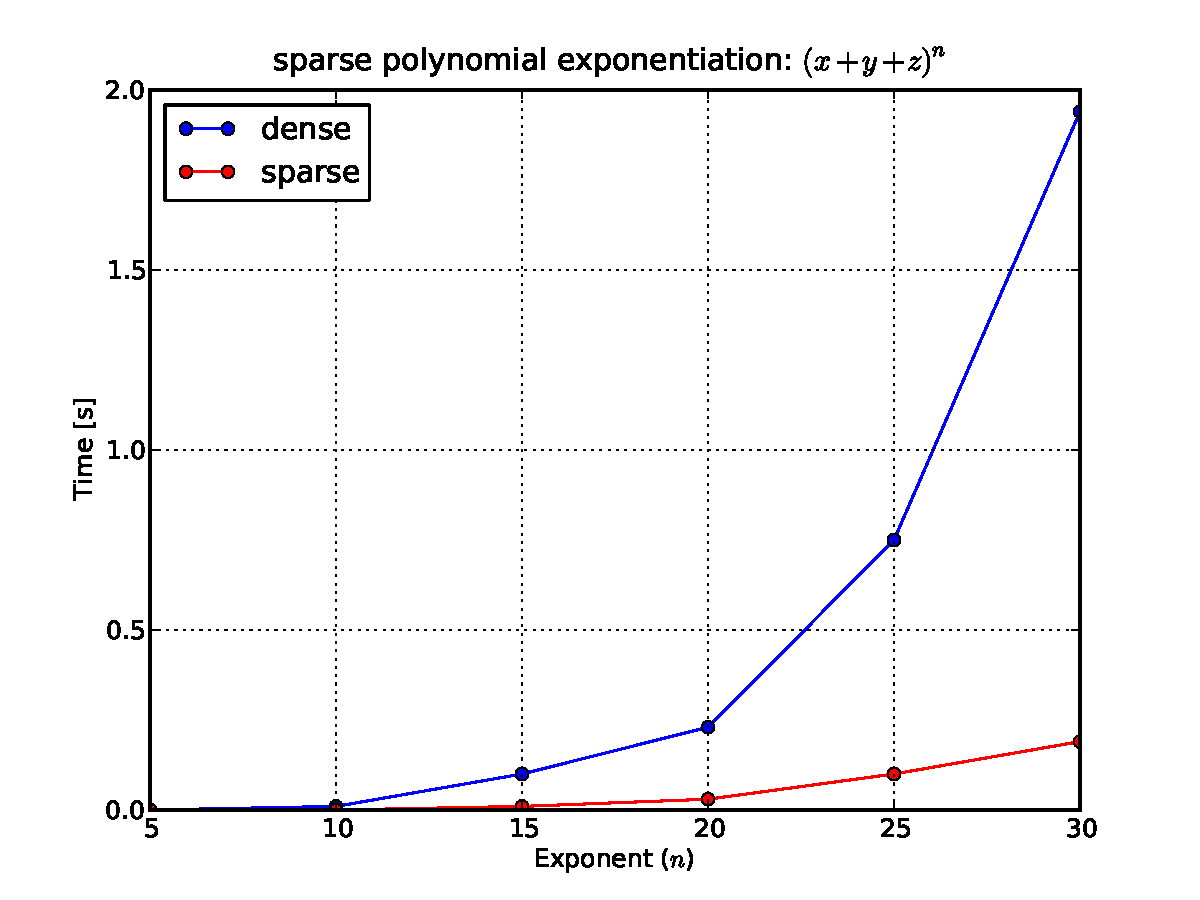
\includegraphics[scale=0.45]{images/sparse-power.pdf}
    \end{center}
\end{frame}

\begin{frame}
    \frametitle{Using pure mode Cython}
    \framesubtitle{An introduction}

    \begin{itemize}
        \item install Cython (\texttt{www.cython.org})
        \item take advantage of \texttt{cythonized} decorator
        \item compile, i.e. wait 20 s (on 1.7 GHz CPU)
    \end{itemize}
\end{frame}

\begin{frame}
    \frametitle{Using pure mode Cython}
    \framesubtitle{Benchmark: polynomial exponentiation}

    \begin{center}
        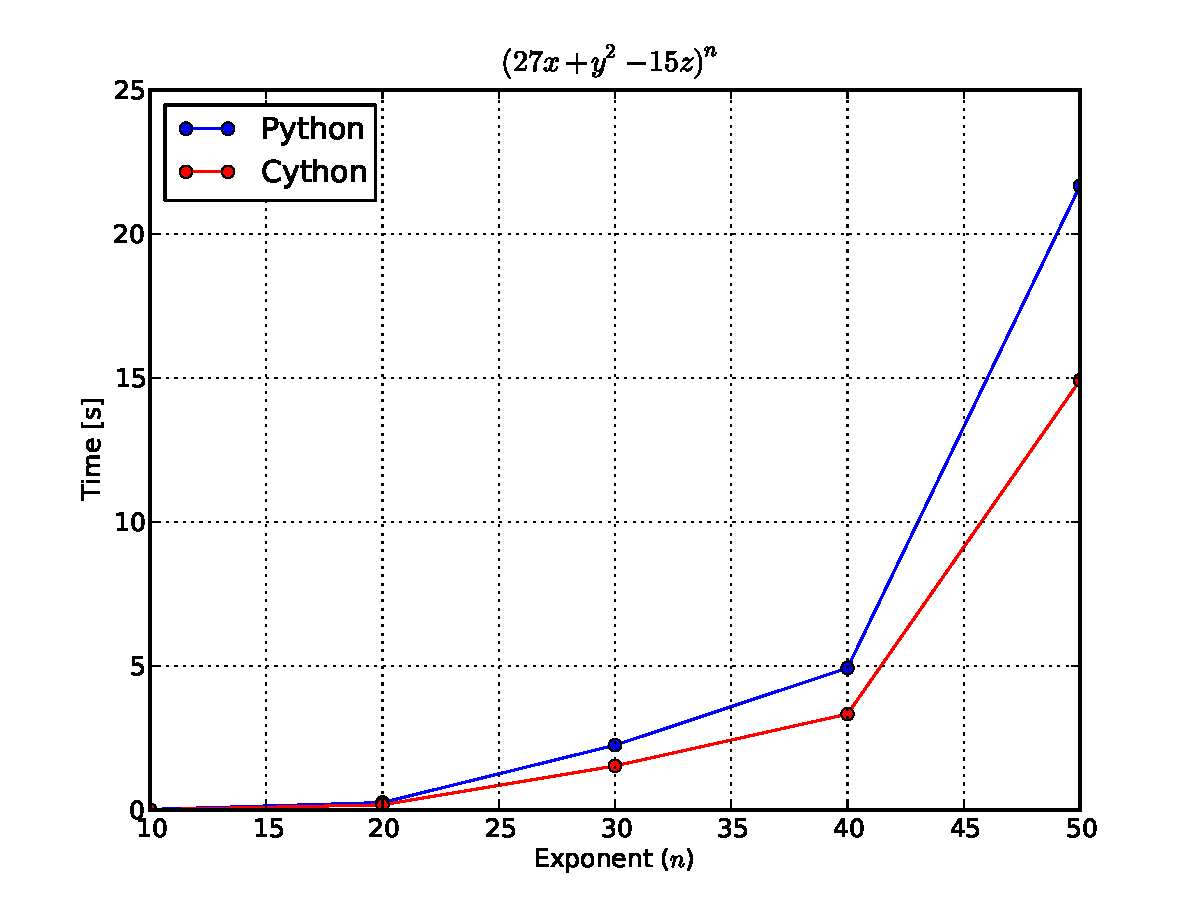
\includegraphics[scale=0.45]{images/cython-power.pdf}
    \end{center}
\end{frame}

\begin{frame}
    \frametitle{Using pure mode Cython}
    \framesubtitle{Benchmark: polynomial factorization}

    \begin{center}
        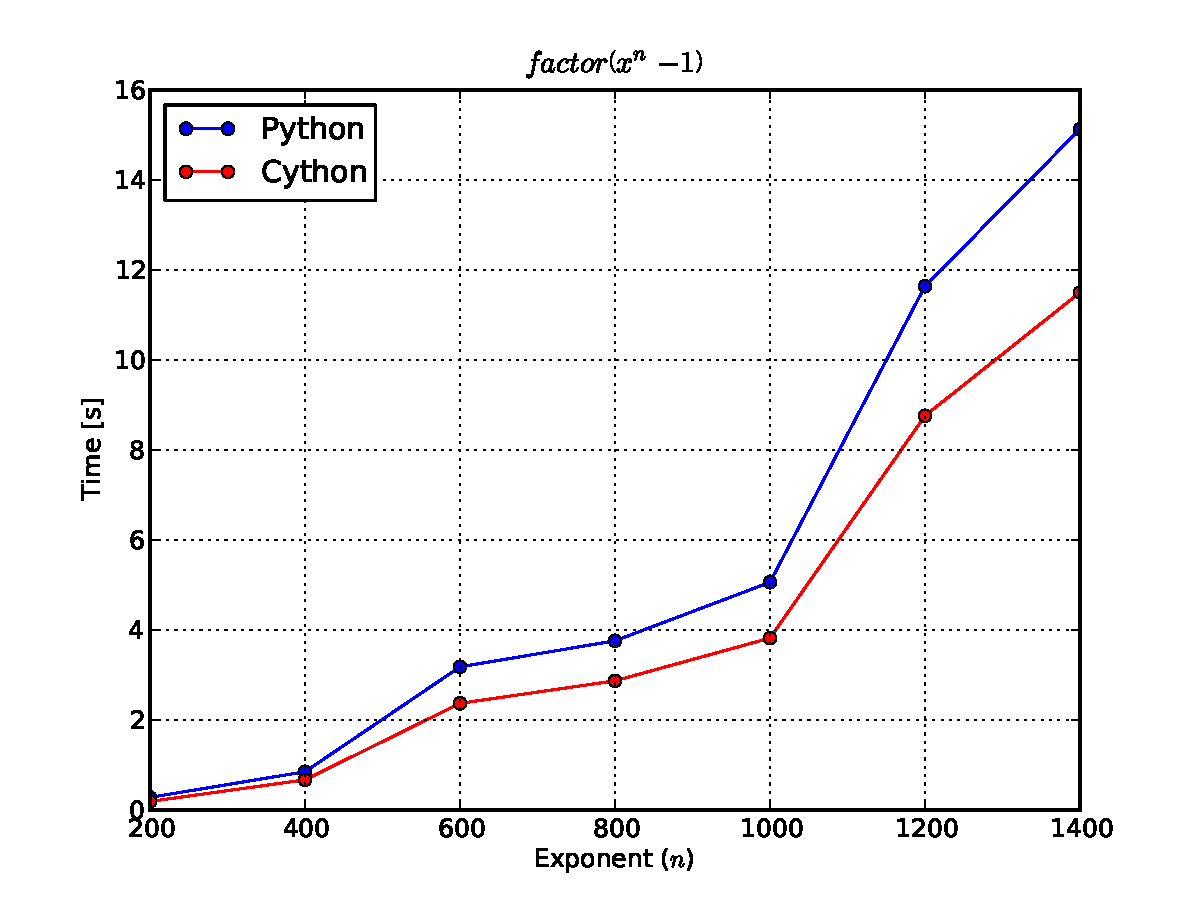
\includegraphics[scale=0.45]{images/cython-factor.pdf}
    \end{center}
\end{frame}

\begin{frame}
    \frametitle{Future plans}
    \framesubtitle{}

    \begin{itemize}
        \item implement better algorithms
            \begin{itemize}
                \item factorization, Gr\"{o}bner bases, \ldots
            \end{itemize}
        \item write more extensive documentation
        \item use the module for pratical things
            \begin{itemize}
                \item GSoC project: Algorithms for Symbolic Integration
            \end{itemize}
    \end{itemize}
\end{frame}

\begin{frame}
    \frametitle{Thank you for your attention!}
    \framesubtitle{Questions, remarks, discussion \ldots}

    \begin{center}
        
\includegraphics[scale=0.2]{images/sympy-logo.pdf}
    \end{center}
\end{frame}

\end{document}

